\documentclass[titlepage, letterpaper, 12pt, oneside]{book}
% --------------------------------------------------------------------------- %
% Comment these lines out to remove the watermark
% --------------------------------------------------------------------------- %
%\usepackage[printwatermark]{xwatermark}
%\newwatermark[allpages,color=red!10,angle=90,scale=3.75,xpos=60,ypos=0]
%{DRAFT\textbullet DRAFT}

% --------------------------------------------------------------------------- %
% fontspec gives problems if you compile with pdflatex
% --------------------------------------------------------------------------- %
\usepackage{fontspec}
\setmainfont{Times New Roman}
% --------------------------------------------------------------------------- %
\usepackage[letterpaper]{geometry}
\geometry{left=1.5in, right=1.25in, top=1.25in, bottom=1.25in}
\usepackage{setspace}
\usepackage{enumitem}
\usepackage{pdfpages}
%\pagenumbering{gobble}
\usepackage{multicol}
\usepackage[section]{placeins}    % Place in a section FORCEFULLY!!
\usepackage{titlesec}             % Important for changing the titles
\usepackage{blindtext}            % Testing
\usepackage{booktabs}             % I can't remember what this is for...
\usepackage{verbatim}
\usepackage{dirtytalk}            % Use \say{thing you want in quotations}
\usepackage{csquotes}             % For block quotes
\definecolor{mtsublue}{cmyk}{1.0,0.44,0,0} % Defines an MTSU blue
\usepackage[breaklinks=true, colorlinks=false, allbordercolors=mtsublue]{hyperref}
\usepackage{url}                  % For urls
\usepackage[labelfont = bf, font = small]{caption} %Allows for use of \caption* for non-labeled captions
\usepackage{graphicx}
\graphicspath{ {images/} }   % Put your images in the images subdirectory
\usepackage{float}
\usepackage[numbers, round]{natbib}
\bibliographystyle{plainnat}
\usepackage{todonotes}
\usepackage{caption}
\captionsetup{width = 0.7\textwidth}
\usepackage{subcaption}

\usepackage{siunitx}
\usepackage{amsmath}
\usepackage{esint}
\usepackage{mathcomp}

\usepackage{listings}
\usepackage{color}
\usepackage{dirtree}

\definecolor{dkgreen}{rgb}{0,0.6,0}
\definecolor{gray}{rgb}{0.5,0.5,0.5}
\definecolor{mauve}{rgb}{0.58,0,0.82}

\lstset{frame=tb,
    language=python,
    aboveskip=3mm,
    belowskip=3mm,
    showstringspaces=false,
    columns=flexible,
    basicstyle={\small\ttfamily},
    numbers=none,
    numberstyle=\tiny\color{gray},
    keywordstyle=\color{blue},
    commentstyle=\color{dkgreen},
    stringstyle=\color{mauve},
    breaklines=true,
    breakatwhitespace=true,
    tabsize=3
}

\pagestyle{plain}
% --------------------------------------------------------------------------- %
% TIKZ STUFF
% --------------------------------------------------------------------------- %
\usepackage{tikz}
\usetikzlibrary{
    shapes,
    arrows,
    decorations.markings,
    positioning,
}

% Define block styles
% --------------------------------------------------------------------------- %
\tikzset{
    startstop/.style ={
        rectangle,
        rounded corners,
        minimum width=2cm,
        minimum height=1cm,
        text centered,
        thick,
        draw,
    },
    io/.style = {
        trapezium,
        trapezium left angle=70,
        trapezium right angle=110,
        text width=2cm,
        minimum height=1cm,
        align=center,
        thick,
        draw,
    },
    process/.style = {
        rectangle,
        text width=5cm,
        minimum height=1cm,
        align=center,
        thick,
        draw,
    },
    decision/.style = {
        diamond,
        text width=5cm,
        minimum height=1cm,
        align=center,
        thick,
        draw,
    },
}
\tikzstyle{arrow} = [
    thick,
    ->,
    >=stealth
]
% --------------------------------------------------------------------------- %

% --------------------------------------------------------------------------- %
% newcommands, newenvironments
% --------------------------------------------------------------------------- %
% Writing
% --------------------------------------------------------------------------- %
\newcommand{\comm}[1]{\textcolor{red}{[#1]}}    % inline comment command

% Math
% --------------------------------------------------------------------------- %
\newcommand{\pprime}{^{\prime}}
\newcommand{\sn}[2]{#1\times10^{#2}}
\newcommand{\snu}[6]{#1\times10^{#2}\,^{+\sn{#3}{#4}}_{-\sn{#5}{#6}}}
\newcommand{\snuwo}[3]{#1\,^{+#2}_{-#3}}
\newcommand{\unitsb}[1]{\,[\text{#1}]}
% --------------------------------------------------------------------------- %

% --------------------------------------------------------------------------- %
% Formatting
% --------------------------------------------------------------------------- %
\renewcommand{\contentsname}{Table of Contents}
\titleformat{\chapter}
    [hang]
    {\raggedright\bfseries\MakeUppercase}
    {\chaptertitle}
    {12pt}{}
    []
\renewcommand{\thesection}{\Roman{section}}
\renewcommand{\thesubsection}{\Alph{subsection}}
\titleformat{\section}
    [hang]
    {\centering\bfseries\uppercase}
    {\thesection}
    {12pt}{}
    []
\titleformat{\subsection}
    [hang]
    {\centering\bfseries}
    {\thesubsection}
    {12pt}{}
    []

\makeatletter
\renewenvironment{thebibliography}[1]{
    \section{References}% <-- this line was changed from \chapter* to \section*
    \@mkboth{\MakeUppercase\bibname}{\MakeUppercase\bibname}%
    \list{\@biblabel{\@arabic\c@enumiv}}%
    {\settowidth\labelwidth{\@biblabel{#1}}%
    \leftmargin\labelwidth
    \advance\leftmargin\labelsep
    \@openbib@code
    \usecounter{enumiv}%
    \let\p@enumiv\@empty
    \renewcommand\theenumiv{\@arabic\c@enumiv}}%
    \sloppy
    \clubpenalty4000
    \@clubpenalty \clubpenalty
    \widowpenalty4000%
    \sfcode`\.\@m}
    {\def\@noitemerr
        {\@latex@warning{Empty `thebibliography' environment}
    }%
    \endlist
}
\makeatother

% --------------------------------------------------------------------------- %
% Author Commands
% --------------------------------------------------------------------------- %
\newcommand{\theTitle}{Testing Methods for Machine Comparison of Real and
Simulated Interacting Galaxy Pair Morphologies}
\newcommand{\theTitlecaps}{\MakeUppercase{\theTitle}}
\newcommand{\theAuthor}{Jackson L. Cole}
\newcommand{\theInstitution}{Middle Tennessee State University}
% --------------------------------------------------------------------------- %

\begin{document}
% --------------------------------------------------------------------------- %
% The following makes equations look much nicer
% \setlength{\abovedisplayskip}{10pt}
% \setlength{\belowdisplayskip}{10pt}
% \setlength{\abovedisplayshortskip}{10pt}
% \setlength{\belowdisplayshortskip}{10pt}
% --------------------------------------------------------------------------- %

% --------------------------------------------------------------------------- %
% Front Matter
% --------------------------------------------------------------------------- %
\frontmatter
\begin{titlepage}
    \begin{center}
        \fontsize{14pt}{16.8pt}\selectfont \theTitle\\
        \vspace{48pt}
        \fontsize{12pt}{14.4pt}\selectfont
        THESIS\\
        \vspace{60pt}
        Presented to the Faculty of the Department of Physics and Astronomy\\
        in Partial Fulfillment of the Major Requirements\\
        for the Degree of\\
        \vspace{36pt}
        BACHELOR OF SCIENCE IN\\
        PHYSICS\\
        \vspace{72pt}
        \theAuthor\\
        \vspace{60pt}
        May 2018\\
        \vspace{60pt}
        \textcopyright 2018 Middle Tennessee State University\\
        All rights reserved.\\
        \vspace{12pt}
        \fontsize{9pt}{10.8pt}\selectfont
        The author hereby grants to MTSU permission to reproduce\\
        and to distribute publicly paper and electronic\\
        copies of this thesis document in whole or in part\\
        in any medium now known or hereafter created.
    \end{center}
\end{titlepage}
\thispagestyle{empty}

\clearpage

%%%%%%%%%%%%%%%%%%%%%%%%%%%%%%%%%%%%%%%%%%%%%%%%%%%%%%%%%%%%%%%%%%%%%%%%%%%%%%%%
%%%%%%%%%%%%%%%%%%%%%%%%%%%%%%%%%%%%%%%%%%%%%%%%%%%%%%%%%%%%%%%%%%%%%%%%%%%%%%%%
% Page 2
%%%%%%%%%%%%%%%%%%%%%%%%%%%%%%%%%%%%%%%%%%%%%%%%%%%%%%%%%%%%%%%%%%%%%%%%%%%%%%%%
\vspace*{24pt}
\begin{center}
    \fontsize{12pt}{14.4pt}\selectfont
    \theTitlecaps\\
    \vspace{24pt}
    \theAuthor\\
    \vspace{216pt}
\end{center}
\begin{flushleft}
    Signature of Author:
    \vspace{4pt}\hrule\vspace{4pt}
    \raggedleft
    \fontsize{10pt}{12pt}\selectfont
    Department of Physics and Astronomy\\
    May 2018\\
\end{flushleft}
\vspace{36pt}

\begin{flushleft}
    \fontsize{12pt}{14.4pt}\selectfont
    Certified by:
    \vspace{4pt}\hrule\vspace{4pt}
    \raggedleft
    \fontsize{10pt}{12pt}\selectfont
    Dr. John Wallin\\
    Professor of Physics \& Astronomy\\
    Thesis Supervisor\\
\end{flushleft}
\vspace{30pt}

\begin{flushleft}
    \fontsize{12pt}{14.4pt}\selectfont
    Accepted by:
    \vspace{4pt}\hrule\vspace{4pt}
    \raggedleft
    \fontsize{10pt}{12pt}\selectfont
    Dr. Ronald Henderson\\
    Professor of Physics \& Astronomy\\
    Chair, Physics \& Astronomy\\
    \vspace{36pt}
\end{flushleft}
\clearpage
\fontsize{12pt}{14.4pt}\selectfont


% --------------------------------------------------------------------------- %
% Abstract
% --------------------------------------------------------------------------- %
\section*{Abstract}
\phantomsection
\addcontentsline{toc}{section}{Abstract}
Although restricted three-body codes are in some cases less physically revealing
than full $n$-body codes in simulating interactions and mergers of galaxy pairs,
they are much faster and more computationally efficient in sampling a large
solution space. For this reason, they are still widely used to reduce the
initial parameter space of merger simulations before proceeding to more
sophisticated, $n$-body models. In this work, we provide \texttt{jspamcli.py},
a user-friendly interface for interacting with an existing restricted
three-body code used in the Galaxy Zoo: Mergers project,
JSPAM \cite{Wallin2016}, and to be used in conjunction with an rendered
image creation and comparison suite which has been co-developed specifically
to integrate with \texttt{jspamcli.py}.

% --------------------------------------------------------------------------- %

% --------------------------------------------------------------------------- %
% TOC, LOF, etc.
% --------------------------------------------------------------------------- %
\tableofcontents
\listoffigures

% --------------------------------------------------------------------------- %
% Main Matter Setup
% --------------------------------------------------------------------------- %
% Setup
\mainmatter
\doublespacing

% --------------------------------------------------------------------------- %
% Content
% --------------------------------------------------------------------------- %
\section{Introduction}
\sloppy
French astronomer Charles Messier's
Catalogue des N{\'e}buleuses et des Amas d'{\'E}toiles (Catalog of Nebulae and
Star Clusters) contains 104 objects visible over the Parisian night sky that
were frequently encountered during his efforts as a comet hunter.
Although compiled in the
eighteenth century and officially published from his personal notes in
\citeyear{Messier},
the positions and characterizations of objects given by \citet{Messier} are
well-enough described that they are all easily and frequently
observed today by amateur astronomers across the planet. One such object carries the following
description (translated from the original French and sourced from
\texttt{http://www.messier.seds.org/xtra/history/m-cat81.html}):
\begin{displayquote}
    It is double, each has a bright center, which are separated
    $4^{\prime}35^{\prime\prime}$.
    The two \say{atmospheres} touch each other, the one is even fainter than the
    other \cite{Messier}.
\end{displayquote}
Of course, in the late eighteenth century, Messier would not be predisposed to
assuming that the \say{very faint nebula} with two touching atmospheres
he describes would be the often-imaged
interacting galaxy pair, Messier 51a and b.
Four years after \citet{Messier}, German philosopher Immanuel Kant only
theorizes that perhaps, the exceedingly dim yet huge \say{stars} are not
stars but seem to be most easily characterized as other Milky Ways \cite{kant}.
The main member of the pair is more colloquially referred to as the Whirlpool Galaxy, which is shown in figure \ref{fig: m51}.

\begin{figure}[h]
    \centering
    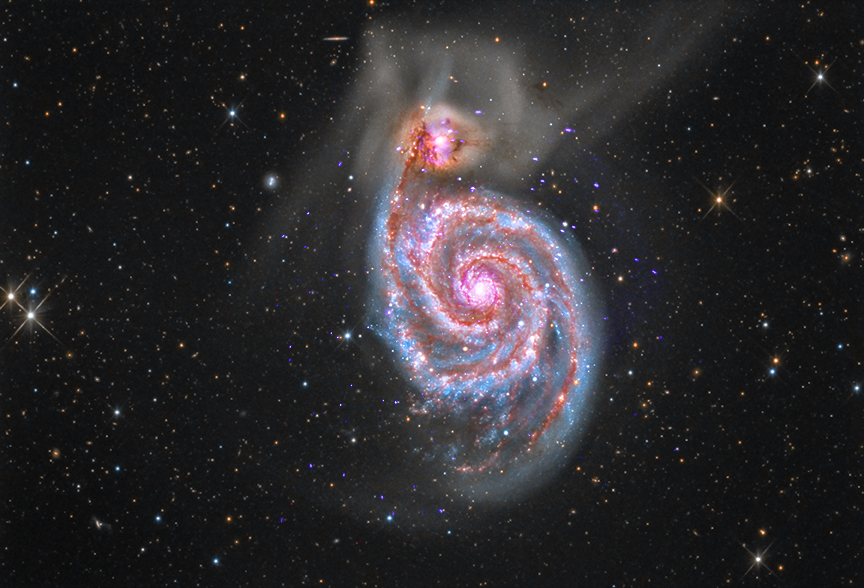
\includegraphics[width=0.5\textwidth]{m51.jpg}
    \caption[Composite image of Messier 51]
    {Composite image of Messier 51, The Whirlpool Galaxy. (Credit:
    X-ray: NASA/CXC/SAO; Optical: Detlef Hartmann; Infrared: NASA/JPL-Caltech)}
    \label{fig: whirlpool}
\end{figure}%


Galaxies are much less frequently found in isolation than they are found
in \textit{systems} of galaxies. We can therefore expect to observe many
cases in which a pair of galaxies are interacting or have interacted in some
way in the history of the system.
Because these interactions are such a common occurrence, a natural
logical next-step is to consider the role which these interactions, or more
narrowly, collisions and mergers, play in the overall dynamics of the system.
\citet{Alladin1965} claimed that collisions between galaxies
drastically increases the internal energy of a particular galaxy and can
potentially lead to changes in overall stellar populations and further,
that the changes in internal structure of galaxies caused by collisions is
significant throughout the observable universe.

Nearly immediately one notices the visually striking and
scientifically puzzling structures of members of an interacting system, as can
be seen in Figure \ref{fig: main}.
These structures are commonly referred to as \say{bridges and tails}
\cite{Toomre1972}.

\begin{figure}[t!]
    \begin{subfigure}[t]{0.5\textwidth}
        \centering
        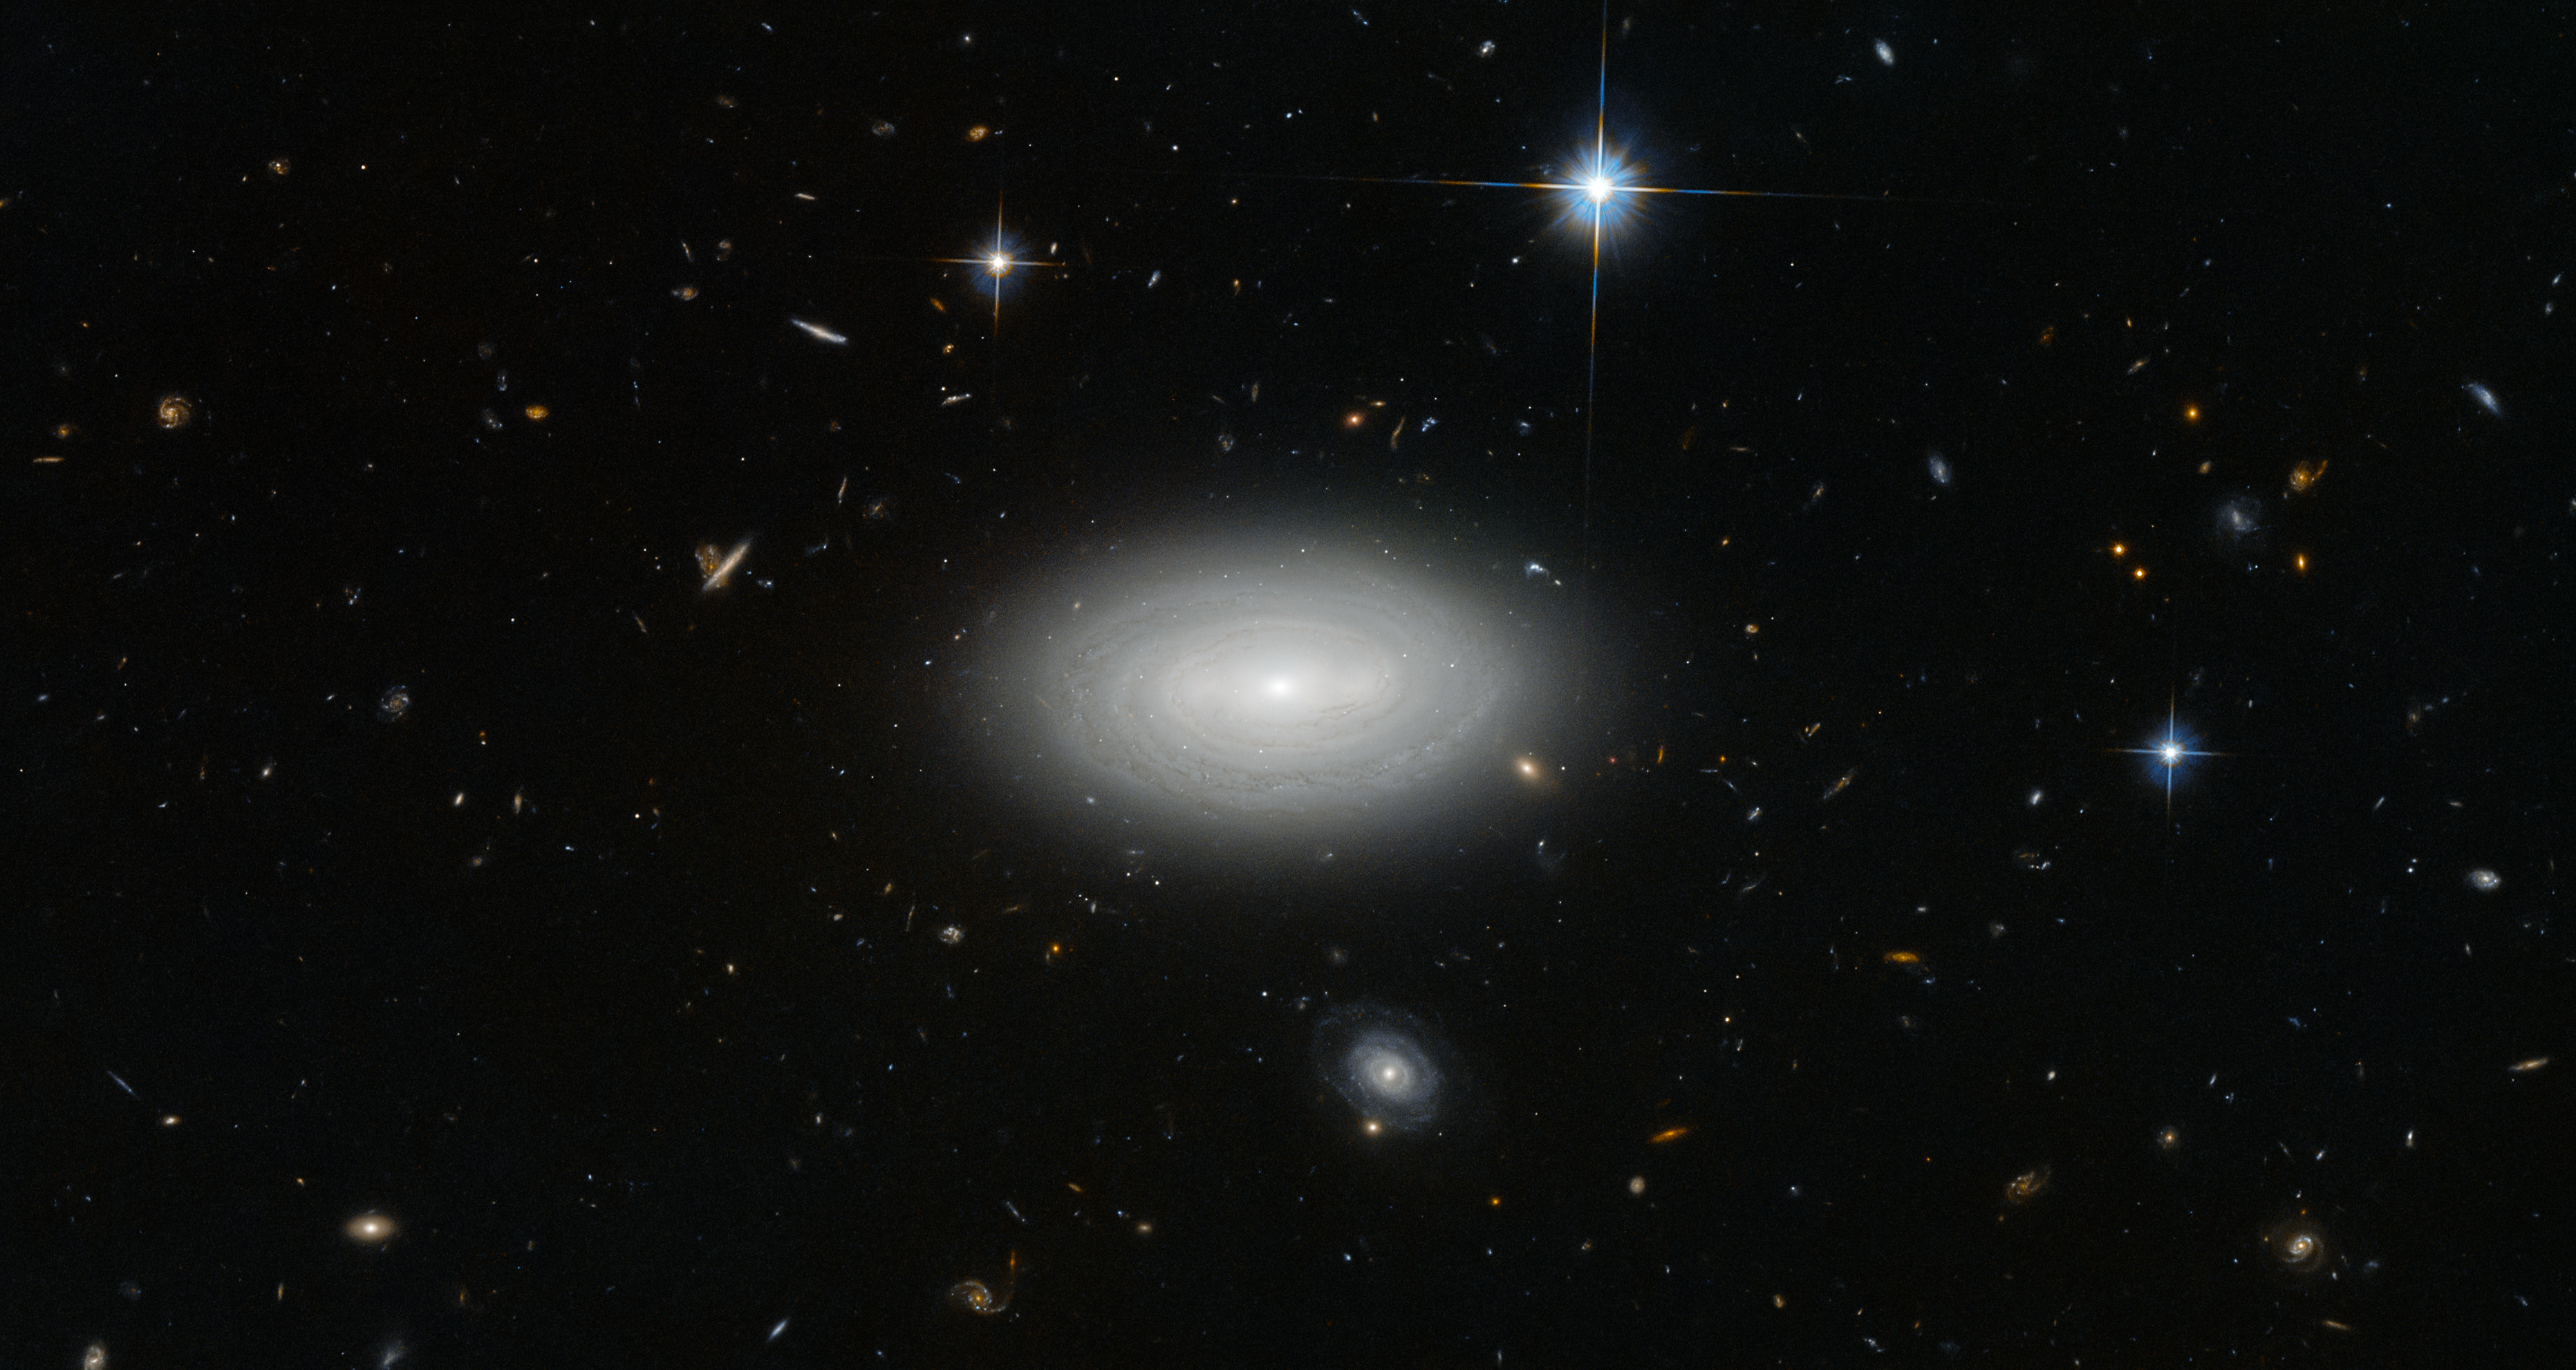
\includegraphics[width=\textwidth]{void.jpg}
        \caption{Example of \textit{undisturbed} morphology, MCG+01-02-015
    (Credit: ESA/Hubble \& NASA and N. Gorin (STScI))}
    \label{subfig: void}
\end{subfigure}%
~
\begin{subfigure}[t]{0.5\textwidth}
    \centering
    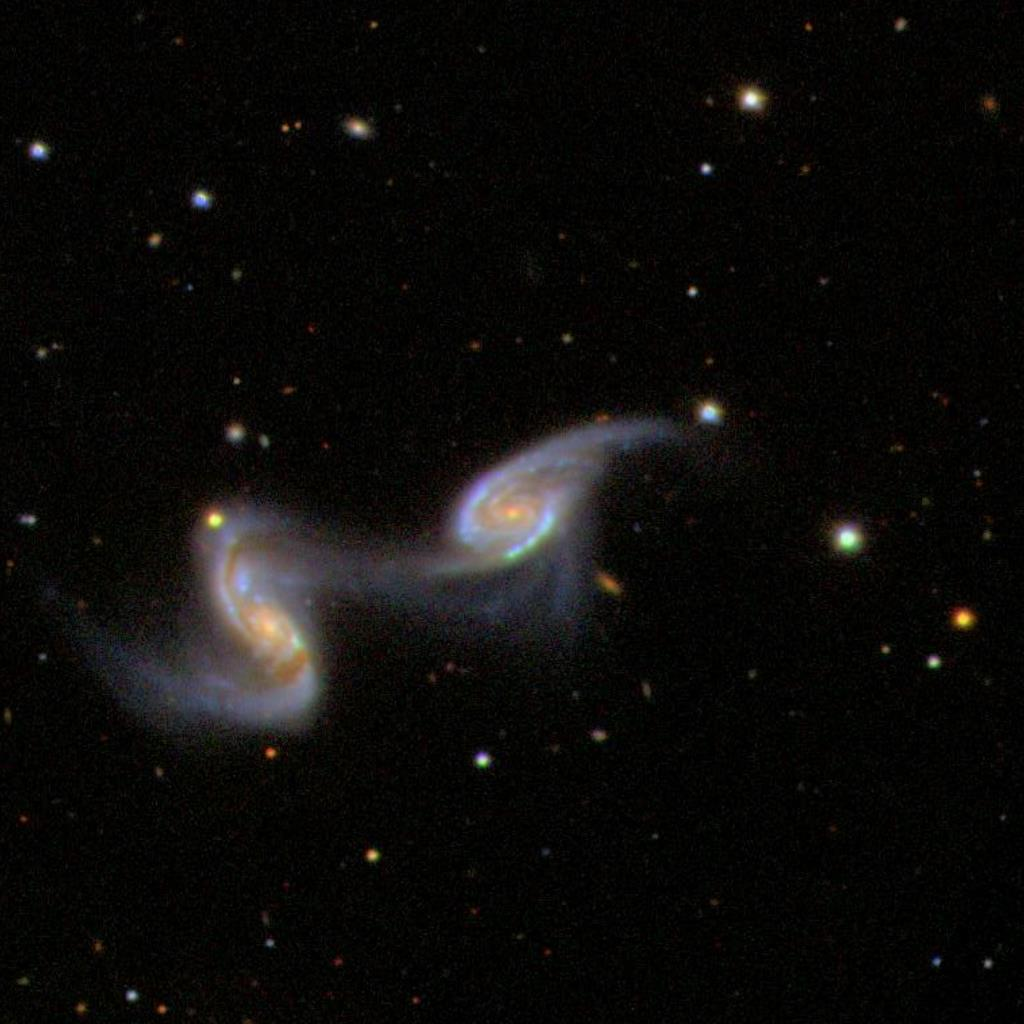
\includegraphics[width=\textwidth]{main_target.jpg}
    \caption{Example of \textit{disturbed} morphology, SDSS DR7 image of
587722984435351614. This target is part of the Galaxy Zoo: Mergers data set.}
\label{subfig: main}
    \end{subfigure}
    \caption[Comparison between undisturbed and disturbed
    morphologies]{Comparison between undisturbed and disturbed morphologies}
    \label{fig: main}
\end{figure}

Optical and spectroscopic observations can readily yield accurate measurements
of the final positions of the galaxies in a merger, and occasionally the radial
velocities of the members of a system can be observed as well. However,
the primary interest
lies in the mechanisms that result in the observed bridges and tails; this
immediately suggests the need to find precisely the final positions in space,
the overall velocity field of system, and the angular orientations of the system
with respect to our position in space. For this reason, much work has been done
in the last 70 years to advance simulations of interacting systems, and further,
to optimize the existing simulations for better convergence on solutions.


%\todo[inline]{
%  \textbf{ITEMS TO CONSIDER ADDING TO INTRODUCTION:}
%  Many of these items were discussed after the introduction had been tidied up
%  in its current form. These will be added at a later date once there has been
%  more time to read into these topics.
%  \begin{itemize}
%	\item Typically, starburst galaxies (galaxies that are in the midst of
%	  heavy star formation) are observed in the midst of a merger. Much of the
%	  work done in improving simulations of interacting galaxies is done in
%	  support of research into other mechanisms in galactic evolution; the role
%	  of mergers in changing the distribution of the star population is commonly
%	  referenced as a potential source of star formation.
%	\item Hierarchical mergers in galactic evolution (as in the evolution of
%	  galaxies from their initial generations to those we observe now.
%	  \begin{itemize}
%		\item First generation $\to$ quasars $\to$ AGNs $\to$ modern galaxies
%	  \end{itemize}
%	\item The role of mergers in cosmological evolution as a whole.
%\end{itemize}}


\section{Background}
The primary question regarding observed disturbed morphological features
of interacting galaxy pairs, described as \say{bridges and tails}, relates to
the mechanism by which they were formed.
In 1972, \citet{Toomre1972} presented some of the first widely
accepted supporting
evidence of what they tellingly referred to as \say{old-fashioned gravity}
as a basis for the disturbed morphologies observed in apparently-neighboring
galaxies. \citet{German} provided the
foundation for their work, but their results were largely rejected in the 1950s
and 1960s when the complexities of galactic bridges and tails were assumed to
result from equally complex mechanisms.
During this period, astrophysicists were in some cases vehemently
opposed to using gravitational interactions as the basis of explanation of
disturbed morphological features. However, it was then
shown using restricted three-body simulations of colliding galaxies
that the supposed static nature of transient tidal forces between
members of galaxy pairs matters less when considering the magnitude of the
intensity of those tidal forces~\cite{Toomre1972}.


\citet{Toomre1972} focuses on four simple examples of interacting systems, each
of which serve to illustrate their proposal that the main contributors to the
bridges and tails are kinematic and can be described simply in terms of
gravity.
In each example, they purposely initialize slow,
parabolic encounters between members of the
galaxy pair, as they assume that faster encounters result in thinner tidal
features, and the primary goals of their work focused on proving that gravity
could be one of the sole causes of the observed features.
This immediately seems like an ad hoc initialization, in which
one should find cause for worry that the result may have been biased
towards the desired result. However, they justify their logic by making several
assumptions.

A relatively high frequency of observable encounters of
galaxies traveling along chance, unbound, hyperbolic orbits is
highly improbable, and accordingly,
observational data from many interacting pairs point to their interactions
not having been chance encounters.
It is much more probable that a significant number of interacting pairs were
already bound, and while still highly eccentric, their approach orbits were
still sub-parabolic, meaning that their orbits could readily become bound.
In work the work of \citet{Toomre1972}, a primary disk is initialized that
is composed of a point mass at the center that is surrounded by several
concentric rings of massless test particles.
The secondary \say{disk} is simply a point mass
representing the center of the secondary galaxy. All numerical integrations were
performed separately for each particle in the primary disk, such that the
computational time could be optimized for each particle in the
system~\cite{Toomre1972}. From the work of~\citet{Toomre1972}, it becomes clear
that gravity alone could be a fundamental cause of the observed morphological
features.

In modern times, the primary challenges involved in simulating
interactions between galaxies are not very far removed from those of
computational economy which were highly necessary considerations in the work
of the brothers Toomre in the early 1970s, although we now at least perform
the necessary integration for each particle at each time step.
In many cases, simulations of galactic collisions still make use of restricted
three-body codes similar to those used in the original work in the field.
Restricted three-body codes
only require that the gravitational force between each of the two most massive
bodies in the system and a particular test mass is calculated. These codes work
when the gravitational interactions between each smaller (essentially massless)
test mass in the system is assumed to be negligible in comparison to those
involving the larger masses.
Their primary advantage over their $n$-body counterpart is their computational
economy.
These codes are also still considered valid, as the self gravity of the galactic
disks is assumed to be almost negligible in comparison to the gravitational
interaction of the two galactic centers and each smaller mass~\cite{Toomre1972}.
Of course, computational economy still is a factor, but its role in guiding
the methods for simulations has changed.

Today, the computational power available to researchers
exceeds by far what has been available in the last six decades.
Whereas in decades past, restricted three-body codes were used
primarily on the basis of computational economy, we can now use these same
types of codes as a still-valid method to quickly reduce the size of the
solution space while the space is still populated with
obviously poor solutions.
Essentially, faster three-body algorithms can be used
to accurately simulate more significant kinematic interactions
(e.g.\ those between each point mass and the centers of each galactic disk),
and then fitness-functions,
automatic image recognition and classification via machine learning techniques,
Citizen Science, or some combination of the three can be used to constrain
the solution space to solutions that have a high likelihood of having
reasonable convergence on the actual solution. From the constrained solution
space, full $n$-body simulations can be used for further analysis.

The computational expense of full $n$-body codes is justified by
when simulating the dynamical processes within the disks of galaxies, as these
effects can be accurately simulated for each particle.
If restricted three-body codes, such as JSPAM \cite{Wallin2016}, can be
used to accurately simulate the large-scale kinematic interactions with
reasonable resolution, then they can be used to accurately simulate solutions
across the entire solution space fairly quickly.
From that point, these computationally expensive codes can be used to explore
the reduced solutions space.

In short, we want to make efficient use of computational time
and to reduce the size but increase the complexity of the job left for the
human-in-the-loop.
In recent years, the Galaxy Zoo project used what essentially was a
human fitness-function comprised of Citizen Scientists to review
over three million simulations~\cite{Holincheck2015}.
However, as of writing of~\citet{Holincheck2015}, there existed no general
purpose machine fitness-function for use in determining the level of
convergence of solutions on observed morphologies of interacting galaxies.
This work does not provide a machine fitness-function, but provides tools that
are useful in support of this effort.

This work primarily focuses on developing methods for interacting with JSPAM,
a restricted three-body code originally written in FORTRAN that is described in
\citet{Wallin2016} that can be found at
\texttt{https://github.com/JSPAM-Manga/WallinCode}.
JSPAM simulates these interactions and produces data that can be used to render
the simulated morphologies for eventual use in machine fitness-functions.
However, a standard procedure and pipeline for operating the
JSPAM code and handling the resulting data needed to be developed.


\section{Methodology}\label{sec: methods}
\subsection{Overview}
\subimport{./methods/}{overview.tex}


\subsection{Image Preparation and Target Data Acquisition}
\subimport{./methods/}{image_prep.tex}

\subsection{Targets and Target Input Files}
\subimport{./methods/}{targets.tex}

\subsection{\texttt{merger} Package}
\subimport{./methods/}{merger_package.tex}

\subsection{Naming and Storage Conventions}
\subimport{./methods/}{naming_and_storage_conventions.tex}

\subsection{JSPAM Command Line Interface (\texttt{jspamcli.py})}\label{subsec:jspamcli}
\subimport{./methods/}{jspamcli.tex}

% ---------------------------------------------------------------------------- %
%\subsection{JSPAM, Restricted three-body Simulations}\label{ssec: jspam}
% ---------------------------------------------------------------------------- %
%\todo[inline]{I was not able to add any review of restricted three-body
%    simulations as of yet. I will be adding more information here, as they are
%    essential for cutting down on computational time when the parameter space
%    is still too wide for any regular, beneficial, simulation of
%non-gravitational physics in full $n$-body simulations.}

%\todo[inline]{For some reason, I did not think to add a description of how the
%    actual simulation is run, as we did not write the simulation. Readers would
%    benefit from having this information included. I will be adding this in the
%future.}


% ---------------------------------------------------------------------------- %
% COMMENTED OUT
% ---------------------------------------------------------------------------- %
\begin{comment}
\subsection{Fitness-function Development}\label{ssec: fitness}
The primary goal of this work as a whole is to make progress on the
development of a fitness-function that will return some kind of machine score.
If we find an efficient method for determining convergence of models on the
observed morphologies that rivals that of a human fitness-function, we can then
begin using this method for real-time analysis of models. Although human
fitness-functions are robust and can make use of our innate pattern-matching
abilities \cite{Holincheck2015}, the ability to determine model convergence more
precisely with improved fitness-functions in
sequence with simulations immediately opens the door to improving the results
of previously applied genetic algorithms and applying new machine learning
techniques for optimizing the parameter space for all possible solutions.

That being said, we would be \textit{wrong} to not acknowledge the innate pattern-recognition abilities of humans that made the success of the Galaxy Zoo
project successful \cite{Holincheck2015}.
Rather than abandoning human interaction altogether once
a successful method for machine scoring is in place, perhaps a better approach
is to allow the machine scoring mechanism remove \say{bad} simulations from the
set that needs to receive a human score, effectively reducing the human choice
from the best of \textit{all} solutions to the best of \textit{good} solutions.

\todo[inline]{The current method of comparison is a simple normalization and
subtraction of translated images.}
\end{comment}
% ---------------------------------------------------------------------------- %
% COMMENTED OUT
% ---------------------------------------------------------------------------- %

% ---------------------------------------------------------------------------- %
%\subsection{Fitness-function Analysis}
% ---------------------------------------------------------------------------- %
%\todo[inline]{
%    This section currently has no information because no work has been done in
%    support of this section. Once we have several fitness functions working,
%    we will begin analyzing. I think since this is the primary goal of the
%    project, it really should live in the ANALYSIS section.
%}

%\subsection{Optimization of Initial Parameter Space}
%\todo[inline]{There will be more information added here in future when
%we arrive at this stage in the project, but I think that this will likely be
%better explored in continued research rather than the thesis.}




\section{Results}
The primary objective in carrying out this project was to build an
infrastructure to support the investigation into methods of
optimization of initial simulation parameters based on the output of the
JSPAM simulations.
We have accomplished this objective by establishing a working framework with a
elementary approach at comparison of simulation images and real SDSS DR7, DR8,
and DR9 images prepared with MergerEx.

There now exists a dedicated
\texttt{merger} class with member functions that implement most necessary tasks
relating to the merger data. Rather than deal with data I/O on a case by case
basis, we can now instantiate this class to encapsulate all necessary data for
operations common to analysis of mergers in the context with which we are
concerned. Further, the output from all member functions has been logically
structured to reduce future headaches that come from handling large volumes
of file I/O. There also exist several member functions that aid in visualization
of a particular simulation from start to finish.

The \texttt{merger} class is used extensively in what we dub the JSPAM Command
Line Interface (\texttt{jspamcli.py}). This program makes interacting with
the JSPAM code a bit more intuitive and gives the user several modes of
interaction that we found to be useful in different contexts. Further, we have
now standardized I/O from JSPAM so that future work on the project can rely on
predictable I/O behavior.

We also created an option to execute \texttt{basic\_run} asynchronously across
a variable number of cores. While we have not strictly parallelized
\texttt{basic\_run}, we've distributed its execution to make more efficient use
of powerful workstations that are readily available.


\section{Analysis}
\textcolor{red}{At this point, there are no results to analyze as the project
is still in development.}


\section{Conclusions}
While our goal of establishing an interface for using and
interacting with data from the JSPAM code has been achieved,
it is clear that this work really lies mostly in a support role of other
projects. That being said, successful data-intensive projects rely heavily on
user-friendly data pipelines that handle most of the tedious labor and keep
track of all relevant data in a predictable, well thought-out manner.
We expect that the framework
we have created will be useful in that it lessens the overhead necessary to
bootstrap a project using the JSPAM code for its simulation software by
eliminating the need to create ad-hoc methods for interacting with the
simulation data. At this point, users are instructed on how to best interact
with the software for their needs using \texttt{jspamcli.py}, and there is a
clear method by which the simulation output data is stored and organized.

Because this framework is now well established, it becomes trivial to set
up a batch
run file to produce \textit{all} 66,395 sets of run data and then the
associated rendered images.
Essentially, this gives us a massive set of ranked simulation data that
can serve as a training set for future attempts at improving the results of
JSPAM by applying machine learning techniques.

We recognize near the time of completion of this phase of the project that it
would be quite useful to have a JSPAM interface object that can be used
programmatically and that accepts an initial run string as an argument to a
\say{run} method. In tasks where these initial condition guesses are being
optimized, having an implementation of this would be essential for rapid
testing.

While this project has not arrived at scientific results, we intend for our
code to handle some of the
heavy lifting in future projects electing to use the JSPAM code.

% --------------------------------------------------------------------------- %

% --------------------------------------------------------------------------- %
% Bibliography
% --------------------------------------------------------------------------- %
\clearpage
\bibliography{thesisbib}
% --------------------------------------------------------------------------- %

\end{document}
